\documentclass[12pt,ngerman]{scrartcl}

\usepackage[utf8]{inputenc}
\usepackage[T1]{fontenc}
\usepackage{babel}
\usepackage{tikz}

% Sucht nach minimaltikz.pdf im Netz

\begin{document}

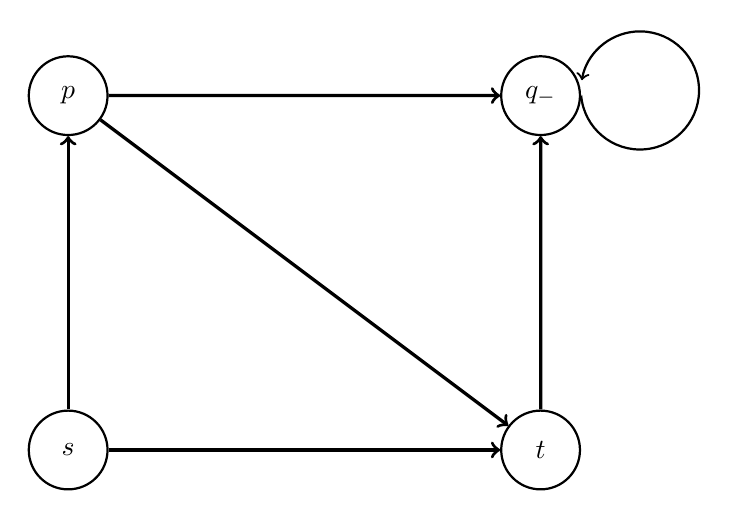
\begin{tikzpicture}[scale=1.5,
    punkt/.style={circle,thick, minimum size = 1cm,draw=black}]
\node[punkt] (s) at (1,1){$s$};
\node[punkt] (p) at (1,4){$p$};
\node[punkt] (q) at (5,4){$q_{-}$};
\node[punkt] (t) at (5,1){$t$};

\draw[->,very thick](s)--(p);
\draw[->,very thick](p)--(q);
\draw[->,very thick](t)--(q);
\draw[->,very thick](p)--(t);
\draw[->,very thick](s)--(t);

\draw[black,thick,->] (q.0) arc (5:350:-5mm);
\end{tikzpicture}


\end{document}